\section{Backlog Plan 2}
\subsection{Description}
For this backlog plan we have the following information:
\begin{itemize}
    \item Plan on 10\% fixing until week 6, when 50\% start to fix troubles, then 100\% after final turnover on week 8
    \item When will the backlog be cleared out?
\end{itemize}
\textit{We are assuming that the team is the same as the previous backlog 
plan, 10 developers, and that the TR fixing rate is still the 
same, 2 TR per week}\newline

\noindent
If the backlog plan is created when will the backlog be cleared out?

\subsection{Process}
The first thing we need to know is what is the percentage of developers fixing 
bugs, according to the descriptions is going to be 10\% until week 6, 
then is going to be 50\% on week 7 and week 8, and after that is be 100\% of 
the developers focus on fixing defects.\newline

\begin{figure}[!htb]
    \centering
    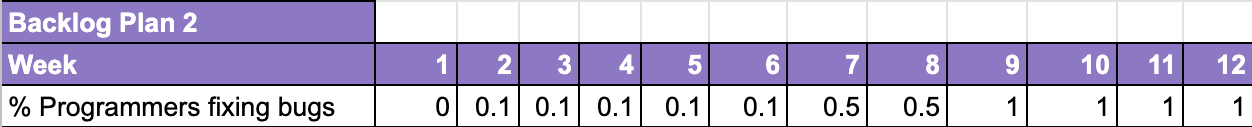
\includegraphics[scale=0.57]{backlog-2-step-1.png}    
    \caption{Programmers fixing bugs}
\end{figure}

\noindent
The next step is to figure out how many bugs are fixed each week, taking into 
consideration the number of developers that are available, we are assuming that 
are going to be 10 developers like the previous backlog and we are also asuming 
that they can fix 2 TR per week.\newline

\pagebreak

\noindent
We calculate this in Figure 9, by multiplying the percentage of developers that
are working each week, by the total amount of developers (\textbf{10}), and we 
multiply that by the amount of TR that they are able to fix 
by week (\textbf{2}).\newline

\begin{figure}[!htb]
    \centering
    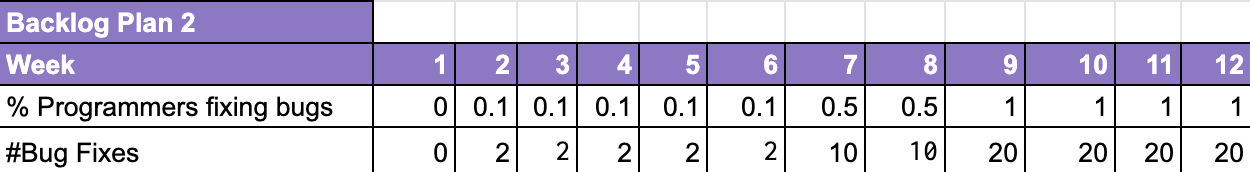
\includegraphics[scale=0.57]{backlog-2-step-2.png}    
    \caption{Bug Fixes}
\end{figure}

\noindent
The last step is to see how many bugs are able to get fixed by the end of each,
we do that by taking the number of defects from the week, subtracting the 
number of defects that the team is able to fix and we add the number of defects 
from the previous week. \newline

\begin{figure}[!htb]
    \centering
    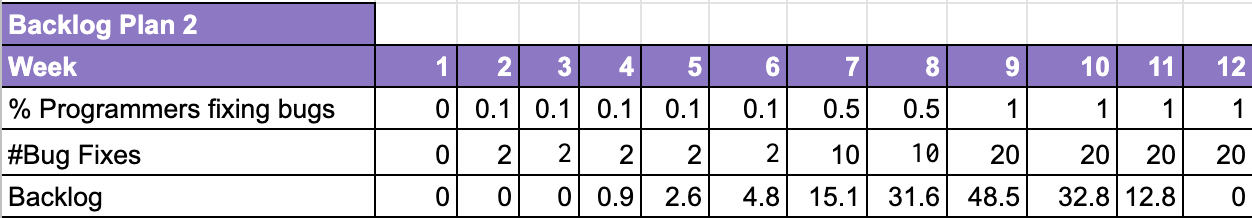
\includegraphics[scale=0.57]{backlog-2-step-3.png}    
    \caption{Backlog}
\end{figure}

\noindent
If for some reason the team is able to fix more defects that the one that 
arrive, we flat the value to 0 because we can't have negative defects fixed

\subsection{Conclusion}
With this backlog approach we are able to clear the backlog in \textbf{12 weeks}.
